\section{Algoritme til detektering af gang, løb og cykling}
\textit{Dette afsnit omhandler design, implementering og test af algoritmerne til detektering af gang, løb og cykling. Først bliver design af algoritmerne behandlet, hvilket er ensbetydende med at implementering og kodning kan foregå. Når algoritmerne er designet og implementeret bliver de efterfølgende testet for at af- eller bekræfte deres virkning.}

\subsection{Design}
For at kunne adskille gang, løb og cykling benyttes et accelerometer og et gyroskop som er beskrevet i \secref{LSM9DS1}\fxnote{opg: tjek op på denne reference}. Herunder vil gyroskopet blive benyttet til at detektere cykling, mens løb og gang detekteres ved brug af accelerometeret. For at kunne detektere og adskille disse aktiviteter, behandles inputtet fra sensorerne gennem forskellig signalbehandling, hvorefter algoritmer afgør om de pågældende signaler repræsenterer gang, løb, cykling eller ingen aktivitet. 


\subsubsection{Gang og løb}
Data fra accelerometerets y-akse skal signalbehandles, førend en algoritme kan detektere og adskille gang fra løb. Første trin i denne signalbehandling er, at fjerne støj ved brug af et elliptisk filter. Dette skal være et fjerde ordens elliptisk båndpasfilter med et pasbånd fra 20 til 50 Hz, og med en dæmpningsgrad på 60 dB\fxnote{og 0.5 dB peak-to-peak ripples}. Båndpasfilterets knækfrekvenser er tildels bestemt gennem pilotforsøget. Knækfrekvensen omkring 20 Hz er enebestemmende for at bibeholde signalets hælnedslag, hvoraf frekvensen befandt sig omkring 20 Hz. Knækfrekvensen omkring 50 Hz er bestemt ligeledes bestemt på baggrund af pilotforsøget, hvoraf signalets frekvensindhold stopper herefter. Andet trin i signalbehandlingen, består af, at det filtrede signal divideres to. Dette er tilfældet da signalets amplituder bliver formindsket, og de mindste amplituder nærmer sig nul i større grad end hælnedslag. Tredje trin i signalbehandlingen består i at det filtrerende og dividerede signal bliver kvadreret. Resultatet heraf medfører at amplituder som er lave ikke forstærkes i stor grad, og større amplituder forstærkes i større grad. Dermed minimeres events som ikke relateres til hælnedslaget kraftigt, og selve hælnedslaget forstærkes.\fxnote{ved gang er det swing og heel strike, ved løb er det primært kun heel strike, men også lidt toe offset.} Fjerde og sidste trin i signalbehandlingen, bliver signalet filtreret med et moving average filter som udglatter signalet, hvilket resulterer i at små udslag ikke opfattes, og signalets hælnedslag vil fremstå som et enkelt event. \\

Førend ovenstående signalbehandling kan overføres til at fastsætte en tærskelværdi skal dataet fra pilotforsøgets data omregnes til LSM9DS1' arbejdsområde: 
\begin{equation}
\frac{32 g \cdot 2^{16}}{32 g \cdot 2^{12}} = 16
\end{equation}
Data fra Shimmer3 samples med en 12 bit ADC, og LSM9DS1 indebærer en 16 bit ADC. Resultatet heraf er at data fra pilotforsøgets skal ganges med 16 for at repræsenterer LSM9DS1' arbejdsområde.

Resultatet af ovenstående signalbehandling medfører at der findes et udtryk for gang og løbs amplitude forhold. Ud fra denne behandling af pilotforsøgets data vurderes det, at amplituden for hælnedslag ved løb overstiger 1100 og ved gang overstiger 50, hvorfor events med amplituder under 50 ikke vurderes som værende aktivitet.

\begin{figure}[H]
	\centering
	\includegraphics[scale=0.5]{figures/cDesign/algoritme_gl.png}
	\caption{Flowchart over algoritmen til detektering af gang og løb}
	\label{fig:algoritme}
\end{figure}

Ovenstående figur repræsenterer algoritmen for detektering og adskilles af gang og løb. Førend algoritmen tilhørende gang og løb starter, undersøges hvorvidt cykling registreres. Herefter signalbehandles dataene fra accelerometeret, hvorefter der tjekkes hvorvidt der har været inaktivitet tilstede. Hvis dette ikke er tilfældet og løb detekteres, skal en timer stoppe når løb ikke længere detekteres. Når timeren stopper gemmes varigheden for timeren i et array tilhørende udført løb og max peak registreres og gemmes ligeledes. Herefter startes timeren igen. Hvis løb ikke detekteres, undersøges der hvorvidt gang registreres. Hvis gang registreres skal en timer ligeledes først stoppe når gang ikke længere detekteres. Når timeren stopper gemmes varigheden for timeren i et array tilhørende udført gang og max peak registeres og gemmes ligeledes. Herefter startes timeren igen. Hvis algoritmen for detektering af løb og gang ikke registrer aktiviteterne, så bliver der ikke udført nogen bevægelse, og algoritmen starter forfra. \\
Fælles for både detektering af gang og løb er at første målte peak og, eller efterfulgt at inaktivitet kasseres. Dette er tilfældet da dette sikre at en periode med inaktivitet ikke summeres som faktisk gang eller løb. 

\subsection{Cykling}
Data fra gyroskopets z-akse skal signalbehandles, førend en algoritme kan detektere og adskille aktiviteterne. Første trin i denne signalbehandling er at udføre en Fast Fourier Transform (FFT) over fire sekunders sampling. Dette medfører at signalets magnitude og dets tilhørende frekvenser kommer til udtryk, hvorefter andet trin indledes. Dette trin finder den maksimale magnitude med tilhørende frekvens. Tredje trin består af to summeringer, første summering summerer FFT'en fra den frekvens hvor den største magnitude befandt sig $\pm$1 Hz. Anden summering summerer FFT'en fra 1 til 20 Hz. Resultaterne af disse, benyttes til fjerde og sidste trin, som omregner hvor stor en procentdel den første summering udgør af den anden summering. \\
Resultatet af ovenstående signalbehandling medfører at der opstilles et udtryk for signalets spredning af energi. Det gør sig gældende at cykling har en spredning af energi fordelt nært frekvensen med den største amplitude. Data fra gyroskopets z-akse vedrørende cykling blev for alle forsøgspersoner, behandlet med ovenstående metode. Dette resulterede i at 84,5\% til 91,9\% af energien lå $\pm$1 Hz omkring den fundne frekvens. Følgende blev ligeledes behandlet for gang og løb, for at sikre disse ikke havde samme spredning i frekvensområdet, hvormed en mulig tærskelværdi til detektering af cykling, kan fastsættes.  Dette resulterede i at ved gang befandt energien omkring den fundne frekvens sig mellem 35,9\% til 48,5\% og ved løb befandt energien omkring den fundne frekvens sig mellem 42,8\% til 60,5\%. \\
Resultatet af at energien omkring den fundne frekvens med den største amplitude er $\approx$30\% større ved cykling end ved gang og løb, fastsættes tærskelværdien til 70\%. For at detektere cykling skal outputtet fra databehandlingen være større end 70\%.

\begin{figure}[H]
	\centering
	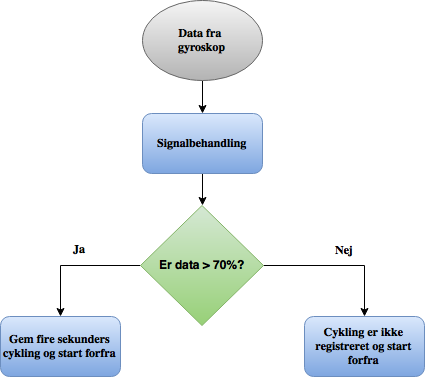
\includegraphics[scale=0.6]{figures/cDesign/algoritme_cykling.png}
	\caption{På figuren ses et flowchart som gennemgår algoritmen vedrørende detektering af cykling. \textbf{DETTE SKAL LAVES OM EFTER VI HAR LAVET ALGORITMEN}}
	\label{fig:algoritme_cykling}
\end{figure}

Ovenstående figur repræsenterer algoritmen for detektering af cykling. Hvis cykling detekteres skal en counter starte og først stoppe når cykling ikke længere detekteres. Når counteren stopper gemmes varigheden af counteren i et array tilhørende udført cykling. Hvis cykling ikke detekteres skal gyroskopet gå i LPM i 10 sekunder før algoritmen køres igen. 


\subsection{Implementering}
\subsubsection{Gang og løb}
Implementeringen af algoritmen for detektering af gang og løb består grundlæggende af to delelementer. Først signalbehandling, hvorefter selve algoritmen implementeres. Signalbehandlingen er blevet implementeret som enestående funktioner igennem C, hvoraf signalet bliver behandlet med fire funktioner førend data bliver kørt igennem algoritmen.

\begin{figure}[H]
	\centering
	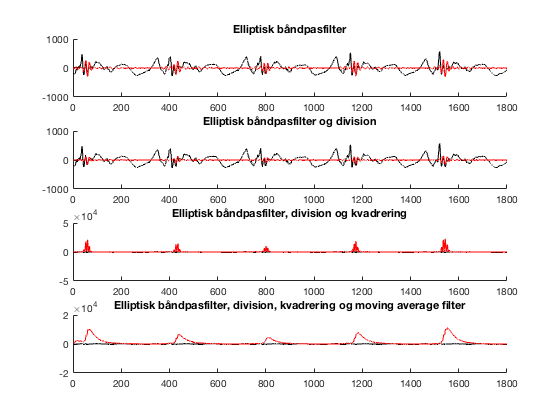
\includegraphics[scale=0.3]{figures/cDesign/signalbehandling_psoc.png}
	\caption{På figuren ses de fire signalbehandlingsfunktioners effekt på rå accelerometer data fra løb. Den sorte kurve på de fire figurer er det rå signal, og den røde er det behandlede output.}
	\label{fig:algoritme_cykling}
\end{figure}

Funktionaliteten af ovenstående signalbehandling sikre at hælnedslag bliver omdannet til en størrelse hvoraf tærskelværdier til detektering er muligt. Det behandlede output antages som værende repræsentativt for hvordan PSoC vil behandle realtids data når det endelige system er færdigt. Dette antages, da det er data fra pilotforsøget, som er blevet behandlet igennem PSoC, og derefter visualiseret. Data fra pilotforsøget er for alle forsøgspersoner blevet behandlet med ovenstående signalbehandling med henblik på fastsættelse af tærskelværdier. 

\begin{table}[H]
	\centering
	\begin{tabular}{ccc}
		\hline
		\rowcolor[HTML]{C0C0C0} 
		Forsøgsperson & Tærskelværdi for gang & Tærskelværdi for løb \\ \hline
		\rowcolor[HTML]{FFFFFF} 
		F1 & 100 & 3000 \\ \hline
		\rowcolor[HTML]{FFFFFF} 
		F2 & 120 & 1100 \\ \hline
		\rowcolor[HTML]{FFFFFF} 
		F3 & 100 & 1100 \\ \hline
		\rowcolor[HTML]{FFFFFF} 
		F4 & 500 & 2400 \\ \hline
	\end{tabular}
	\caption{I tabellen ses tærskelværdierne for forsøgspersonerne vedrørende aktiviteterne gang og løb.}
	\label{tab:individuel_taerskel}
\end{table}
  
De individuelle tærskelværdier er fundet over et fem sekunders vindue. Heraf antages det at tærskelværdierne bør være dækkende for hele målingen, da forsøgspersonerne udførte aktiviteterne ved konstant hastighed.   

\begin{table}[H]
	\centering
	\begin{tabular}{ccc}
		\hline
		\rowcolor[HTML]{C0C0C0} 
		Tærskelværdi for inaktivitet & Tærskelværdi for gang & Tærskelværd for løb \\ \hline
		x \textless 100 & x \textgreater 100 \& x \textless 1100 & x \textgreater 1100 \\ \hline
	\end{tabular}
	\caption{I tabellen ses de tærskelværdier som for alle forsøgspersoner vil kunne adskille gang og løb fra hinanden.}
	\label{tab:faelles_taerskel}
\end{table}

Fastsættelsen af den fælles tærskelværdi bør sikre at gang og løb blandt forsøgspersonerne er mulige at detektere, samt adskille. Igennem behandling af data fra pilotforsøget forekom tærskelværdierne i \tabref{tab:faelles_taerskel} dækkende for alle forsøgspersonerne, hvoraf disse blev valgt.


\subsection{Test}
Algoritmens funktioner testes individuelt samt samlet, ved at indsende et simuleret signal, hvis funktion er at skulle agerer som gang, løb eller inaktivitet. Det simulerede signal er et absolut sinus signal, med varierende amplitude. Amplituden for det simulerede signal afgør, hvorvidt signalet bør agerer som gang, løb eller inaktivitet.  

For at teste algoritmens funktionalitet vedrørende detektering af gang, blev et absolut sinussignal samplet med 512 Hz, en frekvens på 0,5 Hz og en amplitude på 125, indsendt. Dette resulterede i tre halvbølger med en amplitude på 125, på 1536 samples. 

\begin{figure}[H]
	\centering
	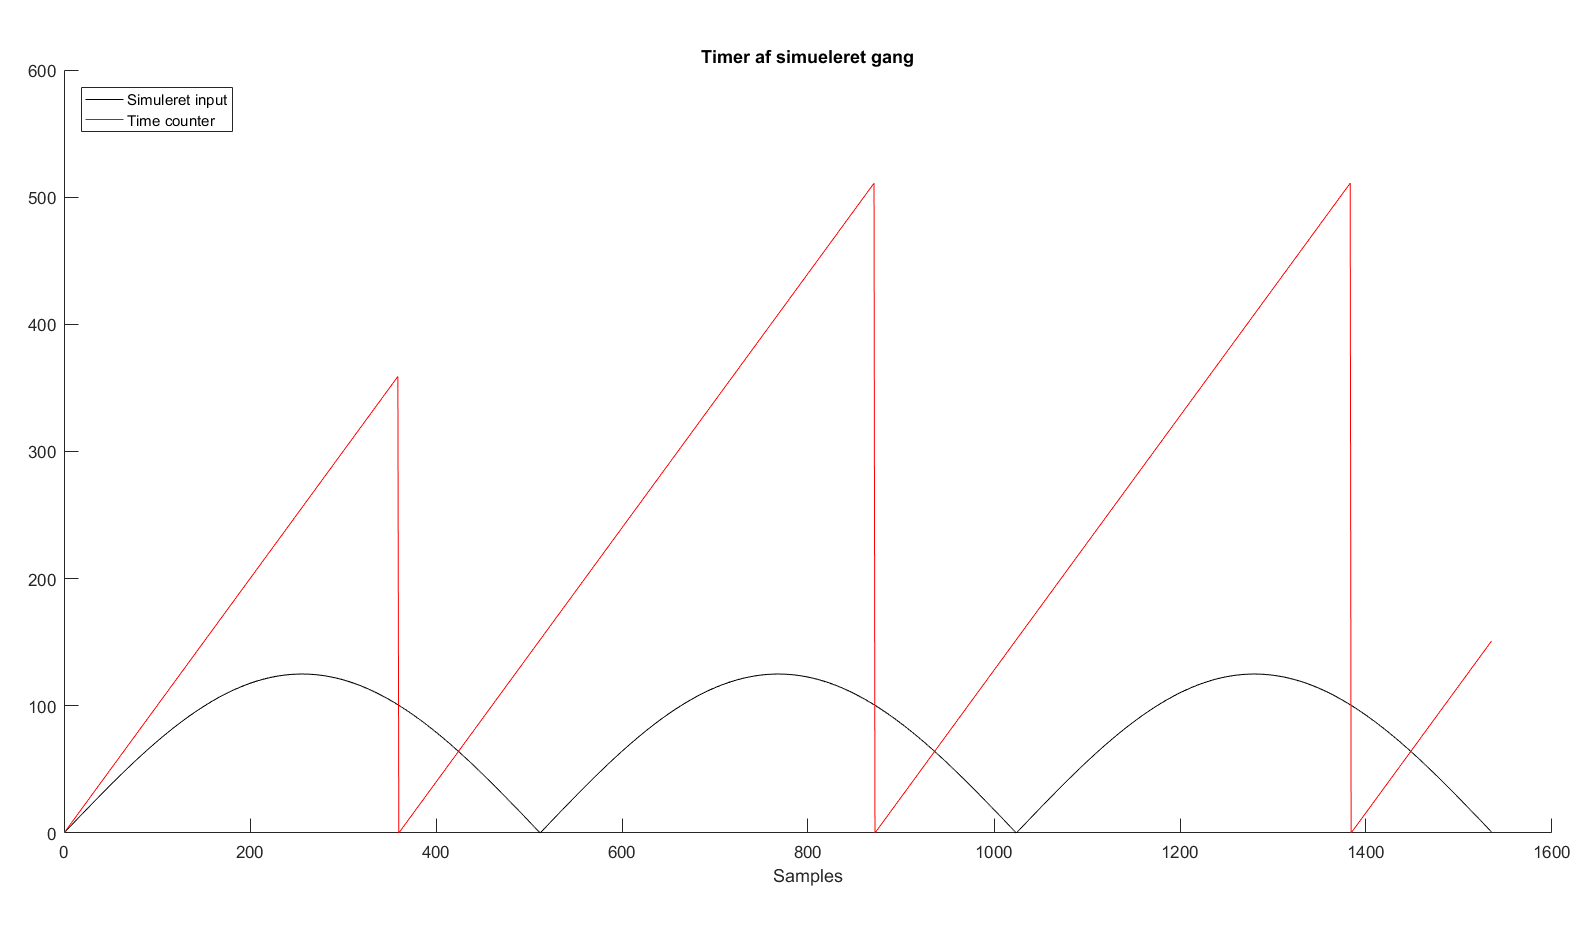
\includegraphics[scale=0.3]{figures/cDesign/test_timecount_gang.png}
	\caption{På figuren ses algoritmens time counter, som resultat af detektering af et gang signal. Den sorte kurve er det simulerede gang signal, og den røde kurve er algoritmens time counter, af samples som overholder algoritmens krav.}
	\label{fig:testgraf_timecounter}
\end{figure}
Algoritmens time counter starter når signalet bliver indsendt, og nulstilles efter en sample, hvis værdi er under tærskelværdien. Heraf kan det ses at varigheden fra at en sample er gået under en tærskelværdi til at en sample igen er gået under en tærskelværdi er 512 samples. En af algoritmens funktioner er at frasortere det første detekterede peak, dermed nulstille time counter værdien, samt peak værdien. Den egentlige test vedrørende algoritmens time counter består dermed i at undersøge hvilke data der videresendes efter et input er kørt igennem algoritmen.

\begin{table}[H]
	\centering
	\begin{tabular}{ccc}
		\hline
		\rowcolor[HTML]{C0C0C0} 
		Værdi videresendt & Forventet værdi [samples] & Modtaget værdi [samples] \\ \hline
		Time counter & $\emptyset$ - 512 - 512 & $\emptyset$ - 512 - 512 \\ \hline
	\end{tabular}
	\caption{I tabellen ses testresultaterne vedrørende test af time counter. $\emptyset$ antyder at det ikke blev modtaget noget ved første peak.}
	\label{tab:test_res_timecount}
\end{table} 
Algoritmen er blevet testet på tre halvbølger, og dermed er det forventede resultat at varigheden af første peak ikke blev medregnet og videresendt som et resultat. Algoritmens time counter fungerede dermed som forventet, og videresendte det forventede resultat. \\

Algoritmens andet resultat som skal videresendes, og dermed en af dets funktioner, er peak detektering. Denne peak detektering er designet således at det ikke skal registrer det første peak i et signal.
\begin{figure}[H]
	\centering
	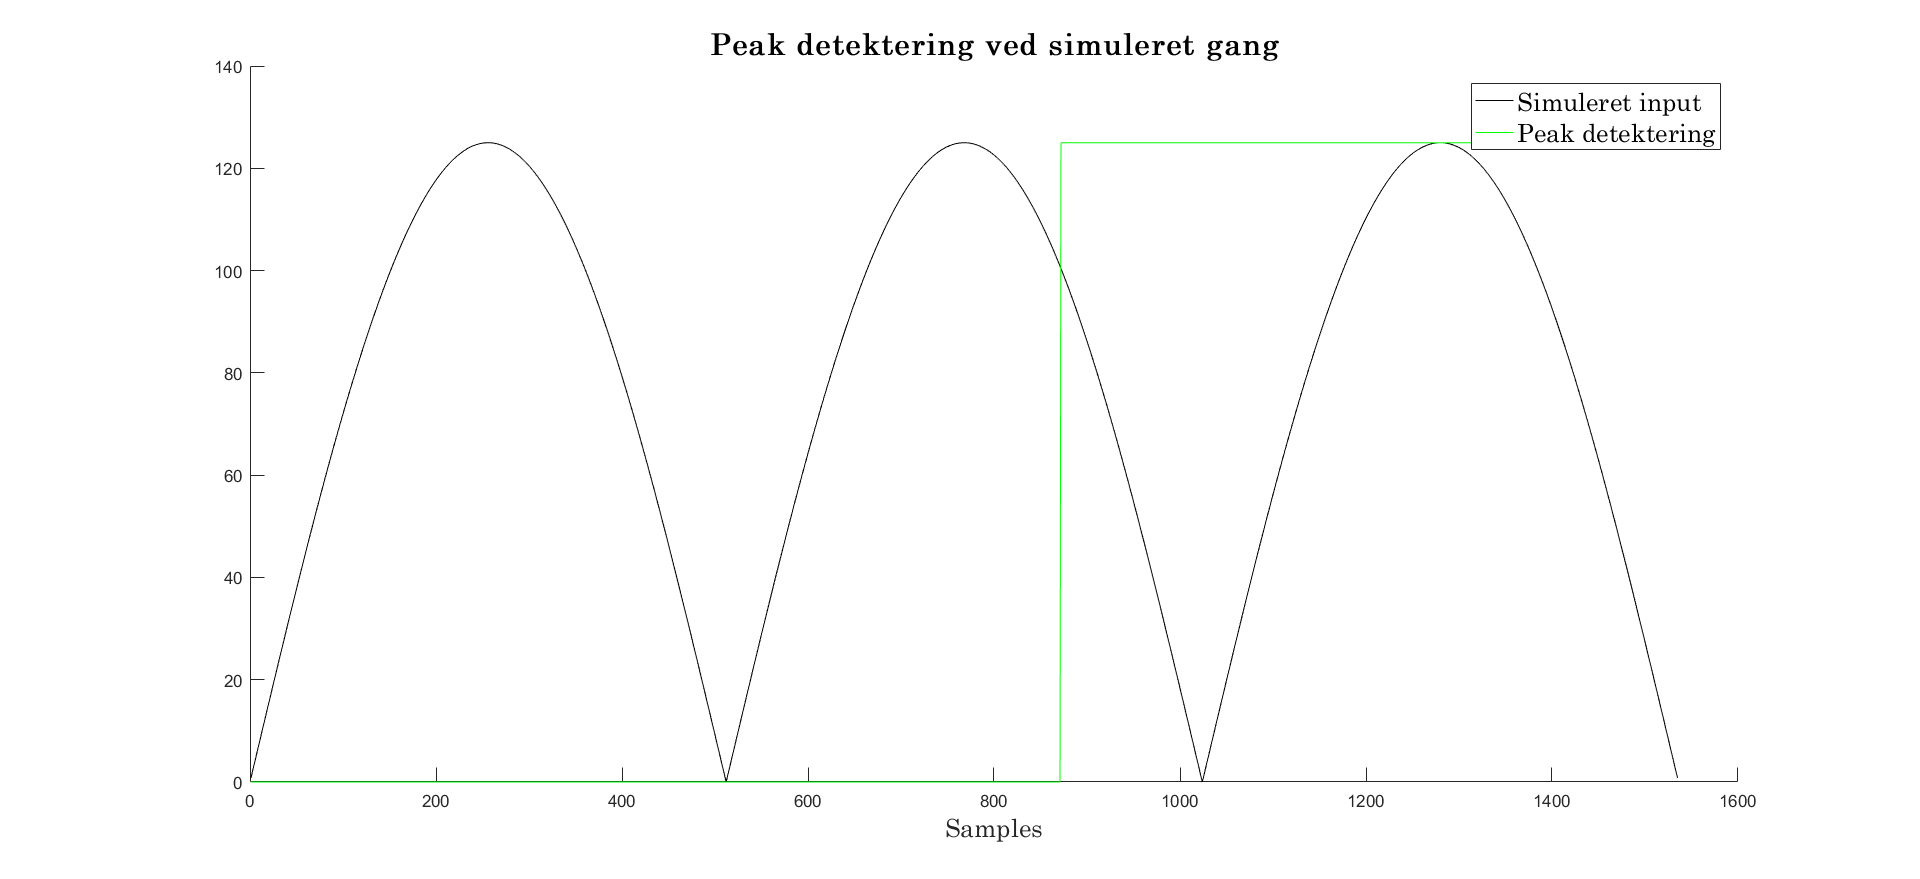
\includegraphics[scale=0.3]{figures/cDesign/test_peak_gang.png}
	\caption{På figuren ses algoritmens funktion til at finde peakværdier, som resultat af detektering af et gang signal. Den sorte kurve er det simulerede gang signal, og den røde kurve er algoritmens funktion til detektering af peakværdier.}
	\label{fig:test_peak_gang}
\end{figure}
Algoritmens detektering af peak starter når en sample overskrider en tærskelværdi, og finder peaket, når en sample er under tærskelværdien. Hvis det er første peak der detekteres sættes værdien til nul. Heraf kan det ses at når samplen går under tærskelværdien anden gang så bliver peaket registreret. Den egentlige test vedrørende algoritmens detektering af peaks, består dermed i at undersøge hvilke data der videresendes efter et input er kørt igennem algoritmen.
\begin{table}[H]
	\centering
	\begin{tabular}{ccc}
		\hline
		\rowcolor[HTML]{C0C0C0} 
		Værdi videresendt & Forventet værdi [samples] & Modtaget værdi [samples] \\ \hline
		Peak detektering & $\emptyset$ - 125 - 125 & $\emptyset$ - 125 - 125 \\ \hline
	\end{tabular}
	\caption{I tabellen ses testresultaterne vedrørende test af detektering af peaks. $\emptyset$ antyder at det ikke blev modtaget noget ved første peak.}
	\label{tab:test_res_peak}
\end{table}
Algoritmen er blevet testet på tre halvbølger, og dermed er det forventede resultat at peakværdien af det første peak ikke blev medregnet og videresendt som et resultat. Algoritmens peak detektering
fungerede dermed forventet, og videresendte amplituden som halvbølgerne var designet med. \\
Algoritmen for løb blev ligeledes testet med henhold til time counter og peak detektering. Ved denne test blev der indsendt et ligende absolut sinussignal, med en anden amplitude som ville overskride tærskelværdien vedrørende detektering af løb. Resultaterne af disse test medførte resultater af samme nøjagtighed som ved detektering af gang. Algoritmen bør dermed fungerer optimalt, både til detektering af gang og løb. 

Algoritmen undersøger hvorvidt data som modtages fra accelerometeret bør klarificeres som værende inaktivitet. Dette gøres ved at indsende et simuleret signal, som først overskrider tærskelværdierne vedrørende gang, efterfulgt af en periode på tre sekunders hvor hverken gang eller løbs tærskelværdi overskrides, efterfulgt af værdier som overskrider tærskelværdierne vedrørende løb. Dette blev testet for både time count og detektering af peak. 
\begin{figure}[H]
	\centering
	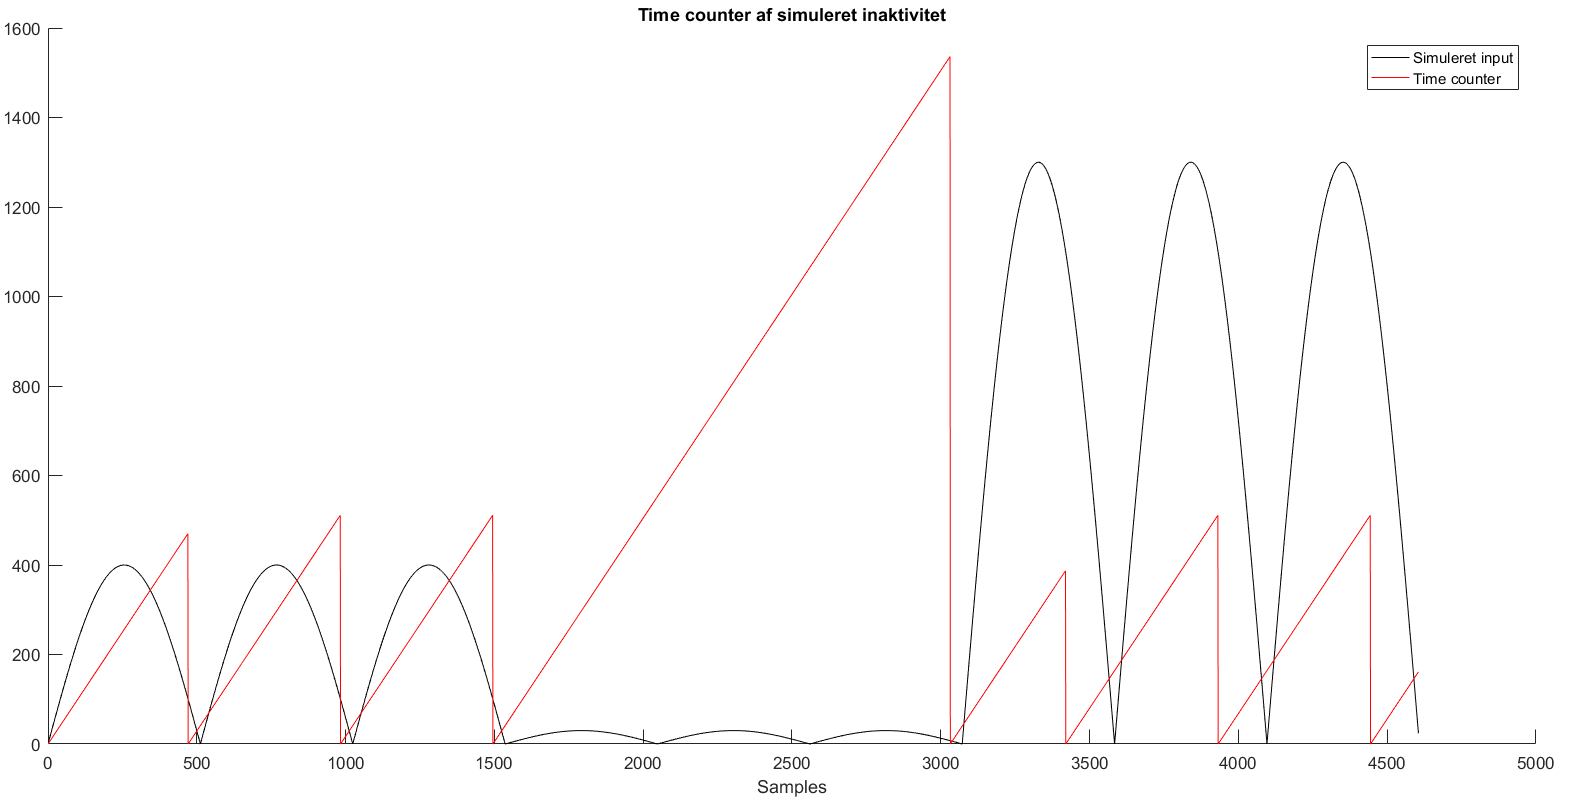
\includegraphics[scale=0.3]{figures/cDesign/test_timecount_inaktiv.png}
	\caption{\textbf{DENNE TEST SKAL LAVES IGEN, MCU HAR IKKE VÆRET NULSTILLET INDEN DEN BLEV KØRT} }
	\label{fig:test_inaktiv_time}
\end{figure}
\begin{figure}[H]
	\centering
	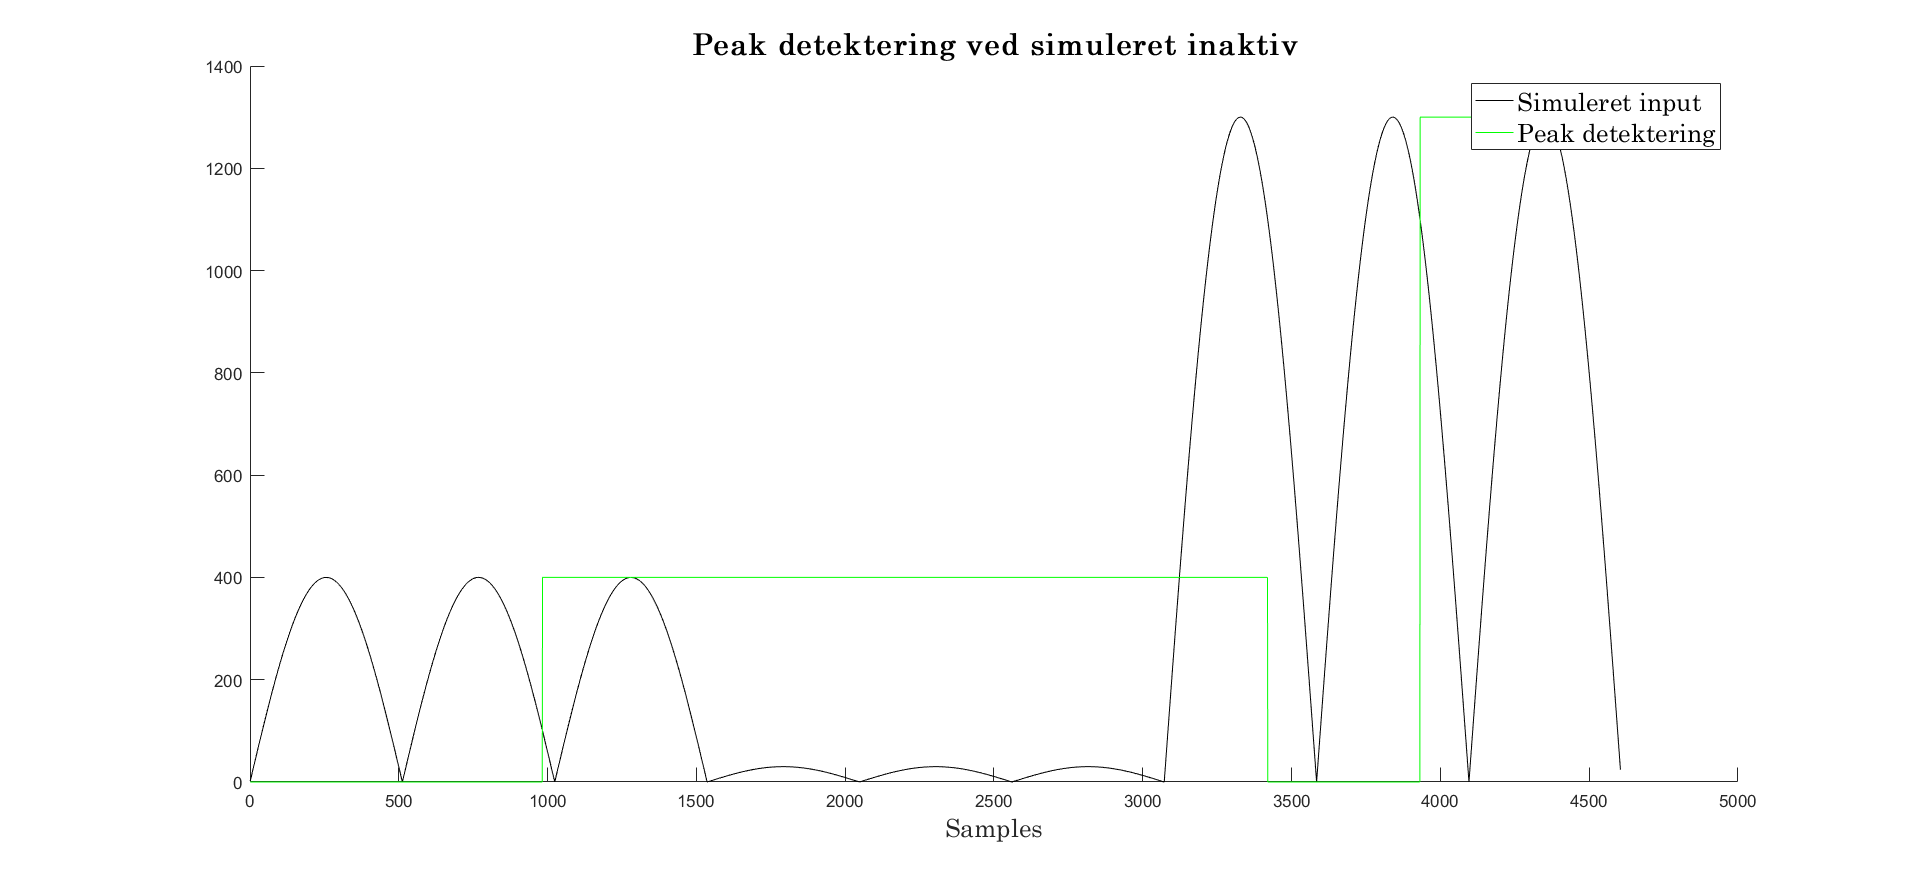
\includegraphics[scale=0.3]{figures/cDesign/test_peak_inaktiv.png}
	\caption{peak}
	\label{fig:test_inaktiv_peak}
\end{figure}
Resultaterne vedrørende time count viser at i perioden med inaktivitet nulstilles time count ikke før en sample har været over og under en tærskelværdi. Resultaterne vedrørende detektering af peak viser at første værdi tilhørende det første peak, samt det første peak efterfulgt af inaktivitet frasorteres. For at klassificere hvorvidt algoritmen omhandlende detektering af inaktivitet fungerer efter hensigten, så undersøges det data som bliver videresendt. Ved et tilfælde med et indsendt input som ovenstående, så bør der registreres to time count værdier med tilhørende peakværdier, efterfulgt af en periode med inaktivitet, hvoraf første peak frasorteres og dermed to time count værdier med tilhørende peak værdier.

\begin{table}[H]
	\centering
	\begin{tabular}{ccc}
		\hline
		\rowcolor[HTML]{C0C0C0} 
		Værdi videresendt & Forventet værdi & Modtaget værdi \\ \hline
		Time counter & $\emptyset$ - 512 - 512 - $\emptyset$ - 512 - 512 & $\emptyset$ - 512 - 512 - $\emptyset$ - 512 - 512 \\ \hline
		\multicolumn{1}{l}{Peak detektering} & \multicolumn{1}{l}{$\emptyset$ - 400 - 400 - $\emptyset$ - 1300 - 1300} & \multicolumn{1}{l}{$\emptyset$ - 400 - 400 - $\emptyset$ - 1300 - 1300} \\ \hline
	\end{tabular}
	\caption{I tabellen ses testresultaterne vedrørende test af time count og detektering af peaks ved et simuleret signal som illustrerer en periode med inaktivitet. $\emptyset$ antyder at det ikke blev modtaget noget ved første peak.}
	\label{tab:test_inaktiv}
\end{table}
Algoritmen er blevet testet på et simuleret signal, som skulle illustrer en periode med inaktivitet omringet af to perioder med henholdsvis gang og læb. Det forventede resultat for både time count værdien og peakværdien er at første peak frasorteres, og første peak efter inaktivitet frasorteres. Dermed forventes det at det videresendte data er time count på 512, og amplituder som afspejler dets design på 400 og 1300. Resultatet af det data som blev modtaget var som forventet, og dermed kan det antages at algoritmens funktion vedrørende detektering af inaktivitet fungerer efter hensigten. 


